
% Large language models (LLM) has demonstrated unprecedented capabilities for knowledge retrieval and content generation across applications~\cite{eloundou2023gpts, bubeck2023sparks, OpenAI2023GPT-4TR}. 
% Software tool manipulation recently emerges as a frontier on the capability of large language models (LLMs) ~\cite{schick2023toolformer,li2023api,qin2023tool}. 
Tool-augmented large language models (LLMs) recently emerge as a research frontier. Such augmented LLMs demonstrate tool manipulation capabilities which automate software operations through natural language instructions~\cite{schick2023toolformer,li2023api,qin2023tool,autogpt,shen2023hugginggpt}. 
% Such tool-augmented LLMs have potentials to automate software-based workflows through a goal description in natural language.
% Tool augmentation emerges as a frontier to enable large language models (LLMs) for software manipulation~\cite{schick2023toolformer,li2023api,qin2023tool}. 
% Such tool-augmented LLMs can automate software-based workflows through a goal description in natural language.
% Such tool-augmented LLMs re-define human-software interactions through natural language description of goals, suggesting omnipresent potentials to automate software-based workflows.
%%% may 13 version
Despite the fact that open-source LLMs substantially shrink the quality gap towards proprietary closed LLMs in tasks such as chatbot~\cite{vicuna2023,openchatkit,laionOA,dolly2dot0}, recent tool-augmented LLMs still mostly rely on closed LLM APIs~\cite{schick2023toolformer,li2023api,qin2023tool,autogpt}. 
% This implies a folklore where open-source LLMs might not be capable enough for tool manipulations, leaving the research and commercial flexibility of these models underutilized. 
% This creates a lack of understanding on the tool manipulation capability of open-source LLMs, leaving their research and commercial flexibility underutilized.
% To alleviate this problem, we ask \emph{can we build on open-source LLMs with minimal human supervision and achieve tool manipulation capabilities competitive to closed APIs}. 
%%% may 14 version
This leads to a fundamental barrier for the industrial adoption of these augmented LLMs due to security and robustness risks associated with exposing enterprise-internal workflows and information to closed LLM APIs~\cite{samsung,jpmorgan}.
To maximize the industrial impact, there is a substantial need for tool manipulation capabilities founded on open-source LLMs. 
To this end, we ask \emph{can we build on open-source LLMs with practical amount of human supervision and achieve tool manipulation capabilities competitive to closed LLMs.}

In this paper, we first demystify key challenges for tool manipulation using open-source LLMs; we then leverage the insights to suggest practical recipes for enhancement. 
% These recipes could inspire research endeavors for open-source tool-agumented LLMs, serving as a stepping stone towards transparent and flexible LLMs for tool manipulation. 
Concretely, we study the setting shown in~\Cref{fig:task_setup} where LLMs take in a natural language instruction as the goal and generate API calls to accomplish the goal. 
Although we expect a quality gap between the open-source and closed LLMs~\cite{liang2022holistic}, what we observe is a far more severe disparity. Specifically, for an on-sale house searching tool, a leading open LLM for code generation fails every test case while the OpenAI GPT-4~\cite{OpenAI2023-ov} attains $77\%$ success rate across the same one hundred examples. 
% Although we do expect some observable quality gap between the open-source and closed LLMs, we unexpectedly observe that representative instruction-tuned open-source LLMs fails every single goal instruction for a trip booking tool while the OpenAI GPT-4~\cite{OpenAI2023GPT-4TR} attains $76\%$ success rate across the same a hundred test cases.  
% In our preliminary experiments, we do expect some quality gap between the closed and open-source models. However unexpectedly we observe that representative open-source and instruction-tuned LLMs fails every single goal instructions for booking trips on a website while the OpenAI GPT-4~\cite{OpenAI2023GPT-4TR} attains $76\%$ success rate across the same a hundred test cases. 
This observation motivates us to study the challenges for open-source LLMs to attain strong tool manipulation capability.

\begin{figure}[t!]
\caption{Tool manipulation setup. 
We augment LLMs as action generators with access to API documentations. 
% Action generators can be plugged into both single-step and multi-step setups. 
% where the only different is if the generated action will be used to interact with a pre-defined environment. 
In a single-step scenario, an action generator directly generates API calls to accomplish the goal. A multi-step action generator iterates with an environment using API calls and generates the next-step calls based on the information from the environment until an exit state.
% The yellow circles are the final results we evaluate. 
% \comment{QT, shall we refer to the background section and make sure key concept are mentioned in this diagram and also caption?}
}
\centering
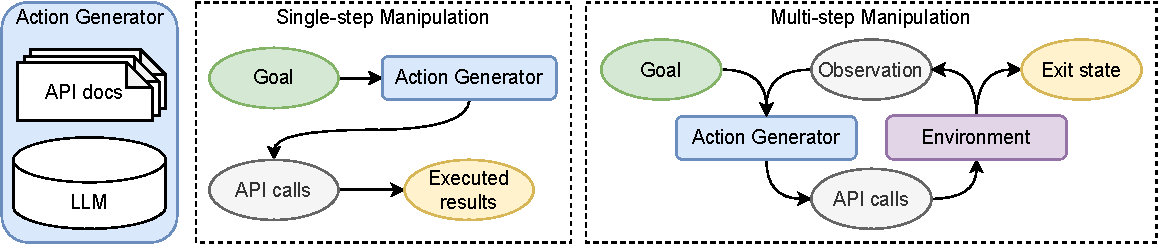
\includegraphics[width=\textwidth]{plots/task.pdf}
\label{fig:task_setup}
\vspace{-1em}
\end{figure}

During our investigation, we identify three key challenges that impede the performance of open-source LLMs in tool manipulation. 
Firstly, open-source models often struggle to accurately identify API names, whereas closed LLMs demonstrate the capability to invoke the correct APIs without explicit usage examples or documentation during inference. 
% Firstly we observe that closed models demonstrate the capability to invoke the correct APIs without example usage or documentations exposed during inference. Meanwhile open-source models encounter challenges even in accurately identifying the API names. 
This suggests that closed LLMs hypothetically internalize knowledge of API usage during training. 
Secondly, we show that without demonstration examples, open-source LLMs often fail to populate the appropriate values for API arguments. 
% test the roofline impact of in-context demonstrations and show that hand-picked oracle examples can substantially alleviate failures in API argument filling.
% Secondly we test the roofline impact of in-context demonstrations and show that hand-picked oracle examples can substantially alleviate failures in API argument filling.
Thirdly, we demonstrate that open-source LLMs tend to produce non-executable generation, such as natural language beyond the desired code. 
% Thus it may require \emph{generation regulation} to only produce executable API calls. 
% Thirdly we demonstrate that open-source LLMs often improperly fill in API arguments 
%  while a hand-picked oracle\footnote{Hand-picked oracle examples are only intended to test the roofline impact of demonstration.} \emph{in-context demonstration} can alleviate. 

Our insights suggest us to revisit three \emph{simple} techniques from LLMs for conventional NLP tasks.
In the context of tool manipulation, 
we adapt them with practical amount of supervision and use them to enhance open-source LLMs.
% the adaptation of such techniques are potentially sufficient to leverage minimal supervision and alleviate major mistakes from open-source LLMs.
% Our insights suggest us to study three techniques \emph{commonly used} in conventional NLP tasks. These \emph{simple} techniques are potentially already sufficient to alleviate major tool manipulation mistakes from open-source LLMs.
\emph{Model alignment:} To first internalize API usage knowledge, we perform instruction tuning~\cite{ouyang2022training,bai2022constitutional} with programatically generated data. Specifically, we first write a few dozens of templates on goals and corresponding API calls. We then pragmatically bootstrap the data volume by instantiating templates with concrete key word values.
% To first internalize API usage knowledge, we perform \emph{model alignment}~\cite{ouyang2022training,bai2022constitutional} through instruction tuning with programatically generated data. Specifically, we first write a few dozens of templates on goals and corresponding API calls. We then pragmatically bootstrap the data volume by instantiating templates with concrete key word values.
% In the template, we provide natural language guidelines to only generate API calls in the desired format. 
\emph{In-context demonstration retriever:} Inspired by retrieval-augmented generation~\cite{borgeaud2022improving,li2022survey,ram2023context}, we additionally enhance the LLMs with a \emph{retriever} to leverage in-context demonstrations during inference. This module selects demonstration examples with the most semantically similar goals from a human-curated pool of examples. Given $n$ API functions, the retriever only requires $\mathcal{O}\left(n\right)$ examples where every API function appears in at least one example. We then leverage LLMs to generalize to goals achieved by unseen API combinations. 
% Inspired by works in retrieval-augmented generation~\cite{borgeaud2022improving,li2022survey,ram2023context}, we additionally enhance the LLMs with an \emph{example retriever} to leverage in-context demonstrations during inference. This module selects API usage examples with the most semantically similar goals from a small human-curated pool of examples. Given $n$ API functions, the retriever only require $\mathcal{O}\left(n\right)$ examples where every API function appears in at least one example. We rely on LLMs to generalize to goals requiring unseen API combinations. 
\emph{System prompt:} Finally we embed goal descriptions into a pre-defined system prompt which provides inference-time guidelines to  generate executable API calls; such system prompts were shown to regulate language style in chatbots~\cite{glaese2022improving}. 
These techniques only require a small amount of human supervision. Thus they render a potentially practical recipe for building on top of open-source LLMs.

To extensively evaluate the inspired techniques, we present \emph{\snact}, a benchmark suite on eight diverse tools ranging from Google Sheets manipulation to controlling robots~\cite{liang2022code}. It enables the first publicly-available quantitative evaluation test bench among the ones brought up in the tool-augmented LLM literature \cite{li2023api, qin2023tool}. For the software tools in our benchmark, LLMs need to accomplish a variety of goals by selecting and combining API functions from up to a hundred candidates. 
%%%%% We additionally create approximately one hundred test cases for each scenario. 
% Users can evaluate LLMs on these cases based on the real software responses in our provided infrastructure. 
% In most scenarios, we also provide a small number of demonstration examples. 
%%%%%% $0.1\times$ to $2\times$ more demonstration examples than the number of API candidates for in-context-learning studies. 
% We release our benchmark for research and commercial purposes.
% making it the first one publicly available for open evaluation on general software tool manipulation.
% We open source the test cases, the evaluation infrastructure and the demonstration examples for research and commercial purposes\footnote{Available at}.

Using the tools in the \snact\  suite, we first empirically show that leading open-source LLMs can demonstrate up to $78\%$ lower success rate when compared to the OpenAI GPT-4 APIs.
% To shrink such gaps, we perform model alignment jointly on all tools using programmatically generated data; we then apply an in-context example retriever and a system prompt during inference. 
We then demonstrate that these simple techniques can substantially improve the success rate of open-source LLMs by up to $90\%$, attaining results competitive or better than OpenAI GPT-4 models in $4$ out of the $8$ tools in our benchmark\footnote{We apply the same system prompt and in-context example retriever for GPT-4. Model alignment is not applicable to GPT-4 as there is no publicly available tuning APIs for it during our experiments.}.
To reveal the impact of different techniques, we provide evidence that aligning model with synthetic data primarily contributes to the significant improvement of open-source LLMs. The system prompt and the in-context demonstration retriever further enhance the performance.
During the enhancement process, we observe that, on average, it takes just one day for a developer to craft the in-context demonstrations and curate the templates for generating model alignment data. This implies that the recipe requires a practical level of human supervision. 

% Regarding the time cost on human supervision, we additionally show that for each benchmark software tool, 
% it only requires one developer approximately one day to craft the in-context demonstrations and curate the templates for model alignment data generation. This implies a practical recipe requiring minimal cost on human supervision. 



% Using our benchmark suite, we first empirically demonstrate that \comment{QT, lets figure out how we want to elaborate the large scale insight validation here.}. We then show that generation regularization with system prompt, minimal in-context demonstration and dedicated instruction tuning for tool manipulation can significantly boost the tool manipulation success rate of open-source LLMs. More concretely, \comment{QT, please complete the concrete claims and observations with numbers clearly discussed here. Make sure we feature with concrete numbers for the fact that the techniques requires very minimal and practical human supervision and compute, and can significantly bump the the success rate.}
% \vspace{-1pt}
Our contributions and the structure of this paper are as follows.
\begin{itemize}[leftmargin=*]
% \begin{itemize}[leftmargin=*, noitemsep]
% \vspace{-5pt}
% \setlength\itemsep{0em}
% \item In~\Cref{sec:insights}, we reveal three key challenges hindering open-source LLMs on tool manipulation.
\item In~\Cref{sec:insights}, we reveal challenges in API selection, argument populating and non-executable generation which hinder open-source LLMs on tool manipulation.
\item To alleviate the challenges, we revisit simple techniques for conventional NLP tasks. We adapt them for tool manipulation to boost open-source LLMs with minimal human supervision in~\Cref{sec:techniques}.
\item In~\Cref{sec:benchmarks}, we introduce the \snact, the first open-sourced benchmark with pre-defined test cases for quantitative evaluation compared to the ones in the recent tool-augmented LLM literature. 
% We release this suite for research and commercial uses.
% \item To evaluate these techniques, we introduce in~\Cref{sec:benchmarks} a benchmark suite on tool manipulation from existing datasets and data we collect. We release this suite for research and commercial uses.
% This is the first open benchmark available for  evaluation on general tool manipulation. 
\item We demonstrate in~\Cref{sec:experiments} that our adapted techniques boost open-source LLMs by up to $90\%$ success rate, showing competitiveness with GPT-4 APIs in $4$ out of $8$ \snact\  tasks.
\end{itemize}
% The rest of this paper is organized as follows. In~\cref{sec:background}, we discuss the problem setup and motivating observations of our study. This is followed by the key empirical insights on the challenges for open-source LLMs in~\Cref{sec:insights}. These insights motivate our techniques for enhancing open-source LLMs in~\Cref{sec:techniques}. We introduce our open-source benchmark suite for tool manipulation evaluation in~\Cref{sec:benchmarks}. We validate our insights across our benchmark and demonstrate the effectiveness of our simple techniques in~\Cref{sec:experiments}. We discuss related work in~\Cref{sec:related} and conclude in~\Cref{sec:conclusion}. \comment{QT, a thoughts here, should we remove the multi step diagram to avoid duplication to algorithm which comes from Tian's comment in better explain the symbols.}



%%%%%%%%%%%%% version Apr 25
% Action generation, as well as the ability to use tools, are the next step in exploring large language models (LLMs) and machine intelligence. To fully unleash the power of LLM, action generation capability is crucial. 
% Although current LLMs have strong comprehension skills, they still lack the ability to judge the confidence of their generated content, and in some cases, they require external tools to obtain more accurate answers in, for example, mathematical calculations and real-time knowledge scenarios. 
% While closed AI models are starting to show more emerging capabilities in action generation, open models are performing poorly them including manipulation of application programming interfaces (APIs). API manipulation is an common and important form of action, and the focus of this work.
% However, there is no standard method to qualify and quantify the action generation capability of LLMs, and there is no comprehesive study comparing different models on different action generation tasks and scenarios.
% Therefore, we want to demystify the challenges that need to be resolved and empower the open-source community and build better open-source models to catch up as "action takers". 

% Our preliminary observations indicate that open-source models are significantly falling behind in the area of action generation. This is problematic, as it could lead to a monopoly of closed models in big tech giants. To address this issue, it is crucial to demystify the challenges associated with action generation using LLMs.
% Demystifying the challenges of action generation using LLMs has the potential to trigger research in the field and encourage the open-source community to push the boundary forward for actions. It could also lead to the development of better open-source models, which could level the playing field with closed models and promote greater accessibility and inclusivity.

% Action Generation is a hard problem that requires strong capabilities in multiple areas, including instruction following and tool-using. Even the most capable LLM out there can still make stupid mistakes on relatively easy tasks and fail on most of the hard problems. Also, API documents and examples are usually long enough to easily exceed the maximum affordable sequence length of a LLM. Thus, an effective information retrieval step is usually necessary for preparing a short enough yet meaningful context for the models. However, the mistakes made in the retrieval steps are usually uncorrectable for the LLM. Furthermore, it is relatively easy to build a complicated pipeline to handle a specific task, but it is necessary and harder to build a universal LLM that only uses zero-shot or few-shot in-context learning (ICL) during inference, to reach high accuracy and reliability. 
% Thus, we need a large enough, realistic enough, diversify enough benchmark suite to evaluate different models and approaches. Additionally, it requires a comprehensive baseline comparison across different models to provide insights on what the key challenges are, especially on those open source models, for API manipulation. We then propose some simple and generalizable techniques from the above insights to trigger and seed the innovation from OSS community.

% In this paper, we present the benchmark we collected, ActGen. It includes 8 real-world tasks, ranging from operating REST API to Python APIs, from controlling software to real work agent, from single step calls to multi-steps calls with environment feedback involved. We also open-source the evaluation framework\footnote{https://github.sambanovasystems.com/SambaNova/web-master}, that can really execute the code generated by the model and check against the expected output. We then provide a in-depth benchmarking and analysis on open source models for key capabilities needed for success. \red{summary of the insights}. These insights motivate us to consider simple techniques on top of open source models, which we show can significantly boost final accuracy. We are also excited to see the community keep contributing and boost the performance and robustness.

% The rest of the paper is organized as follows: 
% We first show how ActGen is constructed to be a comprehensive, accurate and executable action generation database (Section 3). In section 4, we present a comprehensive baseline on ActGen, comparing a bunch of models from open-source communities and closed AI companies, as well as an in-depth analysis of the key features that are required for a model to succeed on those tasks. 
% Our goal is to show that ActGen can serve as a useful resource for action generation tasks with the help of LLMs and other derivative techniques. Then, we proposed several potential techniques in Section 5 that points out several promising direction for the following research.
